% classe del documento
\documentclass[a4paper,10pt]{book}

%package necessari
\usepackage{graphicx}
\usepackage[english]{babel}
\usepackage[utf8x]{inputenc}
\usepackage{verbatim}
\usepackage{amsmath}
\usepackage{hyperref}
\usepackage{listings}
\DeclareGraphicsExtensions{.pdf,.png,.jpg}
\usepackage{graphicx}


% informazioni sugli autori
\author{Dacav, Pietro, Pavel}
\title{Group Editor}

% inzio documento
\begin{document}
\pagestyle{plain}

% parte centrale della copertina
\begin{center} 

\vskip 4cm
\large {First Assignement}
\vskip 1cm
\huge {THE LEGO MOTOR SYSTEM ANALYSIS}
\vskip 6cm
\large {Giovanni Simoni} \\
\large {Pietro Carcereri} \\
\large {Pavel Velychko} \\
\vskip 3cm
\large {Group 1 Editor}
\vskip 2cm
\vskip 1cm
\large {AA 2011-2012}
\vskip 0.5cm
\today
\end{center}


\parskip 12.0pt

\tableofcontents

\chapter{INTRODUCTION}
The system for both the data acquisition and data processing is composed of a Lego Mindstorm and linux o.s. pc. The code language for the brick to be programmed is the c, which is a well known language and permits to the developer a simple debugging process. \\ Once the program has been compiled and uploaded on the brick (instruction on nxtOSEK website), some steps are needed for the data to be transferred. \\
\begin{itemize}
\item launch the BROFist file with the command '-l', this in order to get the bluetooth identification key of the brick;
\item launch the BROFist file with the command '-m' followed by the bluetooth key gets at the previous step, this let the bluetooth data transfer from the brick to the pc (and viceversa) possible;   
\item select the 'BROclient' program and run it by pressing the run button;
\end{itemize}

While the program is running, on the brick monitor is shown information about the software status:
\begin{itemize}
\item name and release of the program; 
\item running phase: every 5 second the motor velocity changes (interval from -100 to 100), this permits to get data from a vast range of velocity;  
\item motor status: information about the motor movement, whether it is running or is not; 
\end{itemize}
The program stops at any time if the ENTER button (that orange) is pressed; this stop the program by invoking the TaskTerminate() method. 

\chapter{DATA ACQUISITION} 
\section{Lego motor (com'e, caratteristiche, approccio)\dots}
So far we have focused our work on the reliability and quality of the bluetooth data transferring. It is a well-known fact that the Lego brick is affected of a delay problems and this makes difficult to receive good data from it. \\ We solved the problem by making the data buffer unidirectional; in other words once our program has been started it stars to send the data to the pc. \\This permits:  

\begin{itemize}
\item a very high reading frequency: (500 hz),
\item high reliability, since the code is integrated directly into the system developed by Michele Bianchi, 
\item a control over the data flow, that permits to manage the inconsistent and redundancy data. 
\end{itemize}

Our program need of the following components in order to work: 
\begin{itemize}
\item LEGO MINDSTORMS NXT Brick;
\item LEGO MINDSTORMS NXT Interactive Motor;
\item Our software, included into the brofist directory;
\end{itemize}
In particular the LEGO MINDSTORMS is an interactive motor what works a 9V with internal gears (overall gear ratio 1:48) that has also an embedded rotation encoder with a resolution of 1?.
\begin{figure} [htb!]
  \centering
 \includegraphics[scale = 0.40]{Graphics/legomotor.png}
 \caption{Picture 1.1. The Lego Motor}
  \label{fig:pos} 
\end{figure}
From this motor it is possible to set two kind of data: 
\begin{itemize}
\item Servo Motor revolution count in degree, by setting a positive or negative value it is possible to make the motor run either in a clockwise or not way.
\item Servo Motor PWM value and brake mode, this value regards the velocity percentage of the motor (if set to zero stops it); 
\end{itemize}



\section{Signal applied to the motor (freq, qualita campioni, grafici \dots)}
  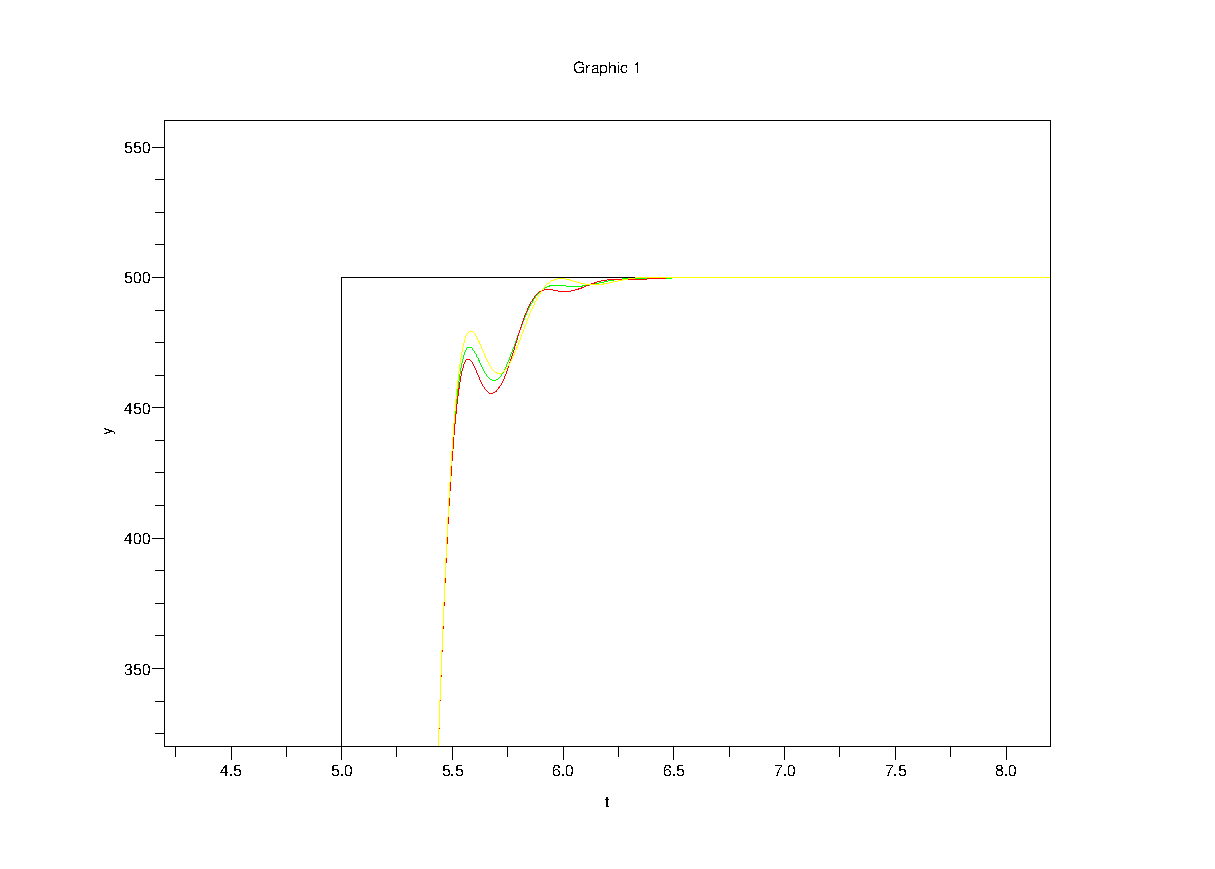
\includegraphics[scale = 0.40]{Graphics/a.eps}



\section{System response frequency\dots}
\section{Challenges and problems\dots}

\chapter{DATA ANALYSIS\dots}
\section{Signal quality (com'era? eventuali adjustements?)\dots}

\section{Step response analysis (steady value, rise time etc.\dots}

\chapter{DATA ESTIMATIONS}
\section{Second order system approximation (dumping factor and sampling frequency)\dots}
\section{Data comparison (fra misurato e reale, grafici++)\dots}
\section{Frequency response analisys (to a sinusoidal signal)\dots}


% Bibliografia
\begin{thebibliography}{9}
\bibitem{pantieri:arte}

Palopoli website \url{http://www.lorenzopantieri.net/LaTeX_files/ArteLaTeX.pdf}.
\end{thebibliography}
\end{document}


\end{document}